\textbf{P3)} Un orgulloso pescador de alta mar cuelga un pescado de masa $65{,}0\ \text{kg}$ de un resorte ideal de masa despreciable. El pescado estira el resorte $0{,}120\ \text{m}$. 

\begin{enumerate}[a)]
\item Calcule la constante de fuerza del resorte $k$.
\item El pescador tira el pescado $5{,}00\ \text{cm}$ hacia abajo y luego lo suelta. \textquestiondown Cuál es el período de oscilación $T$?
\item \textquestiondown Qué rapidez máxima $v_{\max}$ alcanzará el pescado?
\end{enumerate}

\vspace{0.3cm}
\begin{center}
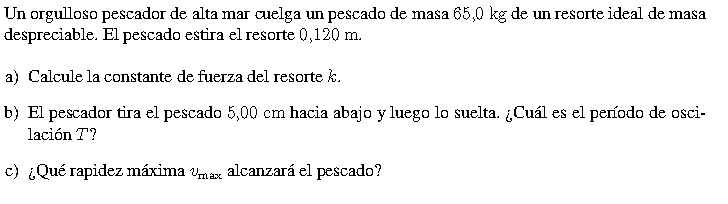
\includegraphics[width=0.62\textwidth]{imagenes/p4a6.PNG}
\end{center}
